Angedacht war \TOWN{San Francisco} mit dem Fahrrad zu erkunden, aber da wir gefühlt in den vorangegangenen Tagen schon alles gesehen hatten, checkten wir zeitig aus und fuhren weiter zur \glqq Farm\grqq.
Eine der ältesten Unis in den USA, die dieses Jahr ihr 125. Bestehen feiert.
War jetzt nicht so besonders, Räume mit Gerätschaften gibt es auch an deutschen Unis.
Da sich die \FOREIGN{Stanford University} inmitten des \FOREIGN{Silicon Valley} befindet, haben 

\begin{tikzpicture}[remember picture, overlay]
\node[inner sep=0pt, yshift=-.25\paperheight] at (current page.north) {%
	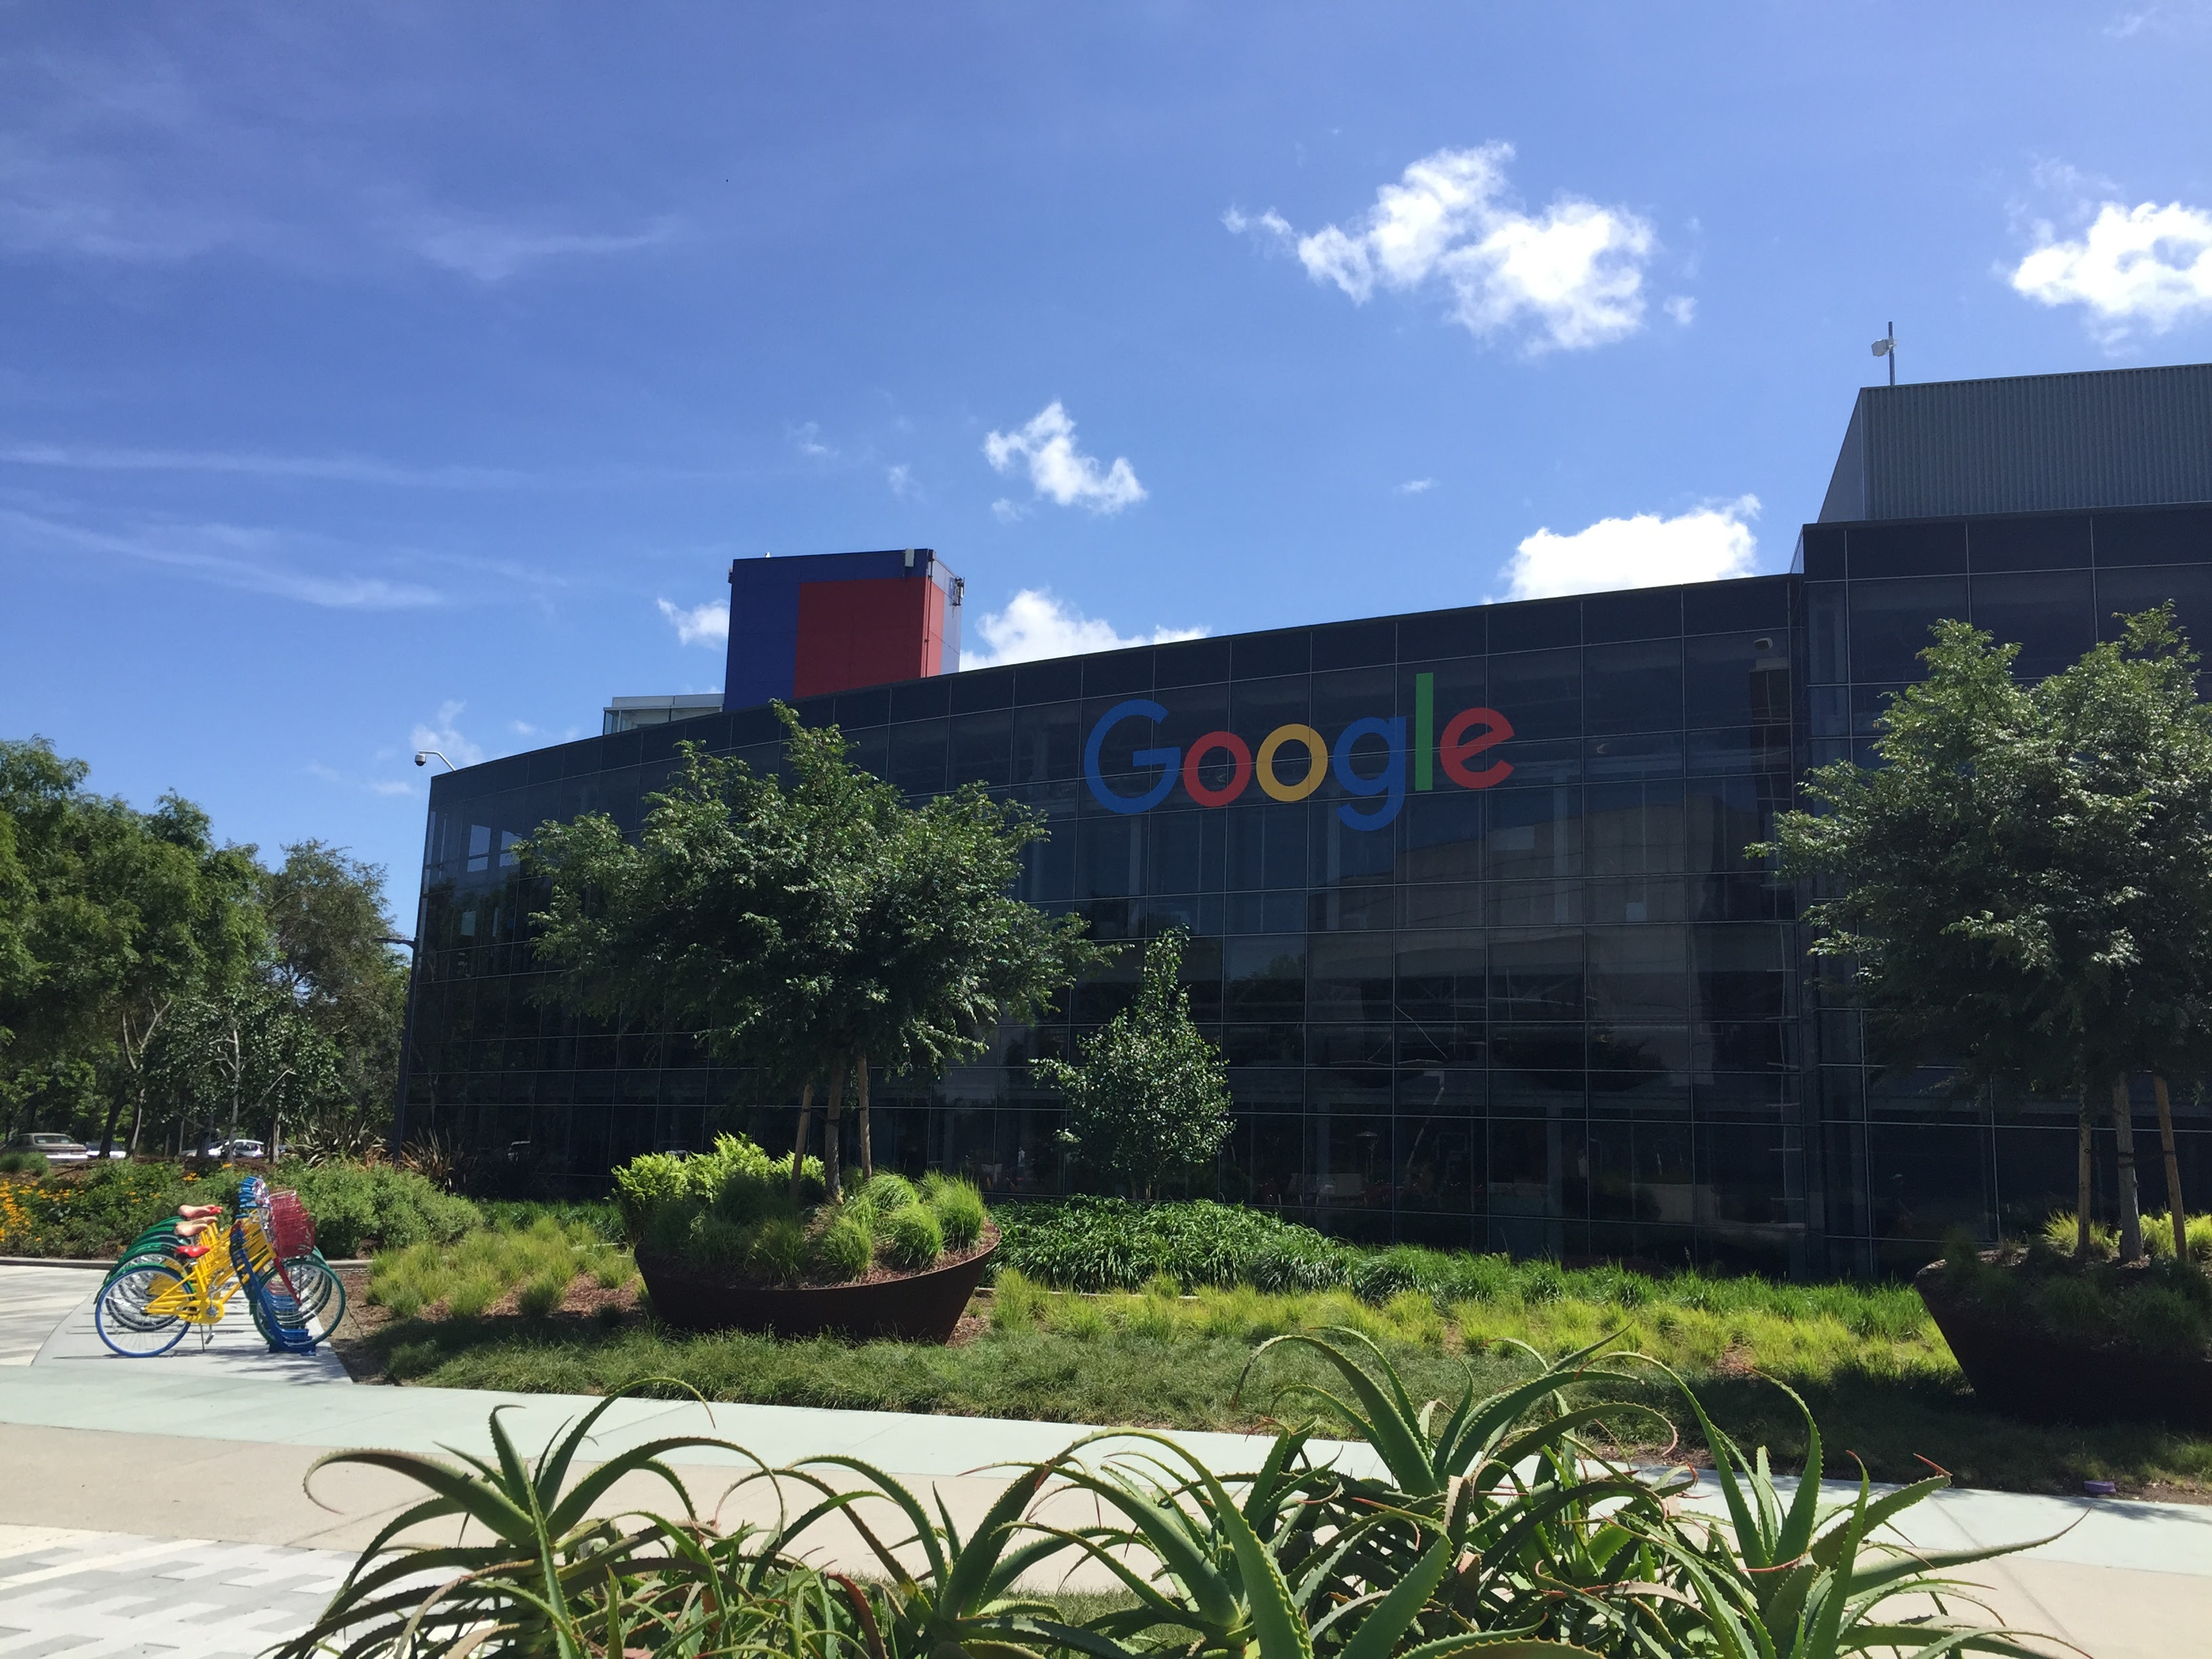
\includegraphics[width=\paperwidth,height=.5\paperheight]{23/google.jpg};%
};
\end{tikzpicture}

\vspace*{.35\paperheight}

\noindent
haben wir noch das ein oder andere IT Unternehmen besucht.
Bei Google war am Wochenende auch nichts los, interessant fand ich nur, dass in die Fläche und nicht in die Höhe gebaut wurde.
Durch Zufall sind wir noch auf einen Deutschen gestoßen, dessen Reisepartner nach vier Monaten Heimweh bekam und der nun die restlichen sechs Wochen alleine herum tourt.

Von \TOWN{Palo Alto} ging es weiter Richtung Yosemite National Park.
Der Weg dahin führte wieder an Plantagen vorbei, im Diner Hula frühstückten wir gegen 16~Uhr (\FOREIGN{Bowl of Oatmeal}\footnote{Haferflocken} und \FOREIGN{Pancakes}) und danach wurde die Landschaft ansehnlicher.
Erst hügeliger, dann richtig bergig.
Die \glqq Passstraße\grqq \, war wahnsinnig schön!

Im Hostel \TOWN{Groveland} genehmigten wir uns zu zweit ein achter Zimmer (45~\$ statt 35~\$).
Der Weg zu den Betten führte durch die Küche und in dieser werkelte ein französisches Paar mit dem Resultat, dass die ganze Hütte nach ihrem Essen roch.
Auch noch am nächsten morgen.
Da hatte sich das Waschen der Wäsche am Abend ja gelohnt.
Am Abend besuchten wir noch die älteste Kneipe Kaliforniens den ``\FOREIGN{Iron Door Saloon}''.
Dort gab es was zu Essen, Livemusik und zu unserem Glück ein Paar, dass voll wie die Haubitzen war und Platz für uns machte.
Zu Essen gab es Burger, zu Trinken ein Dunkel das schmeckte!

Im Verlauf des Abends erzählte mir die \glqq Anführerin\grqq \, der \FOREIGN{Bachelorparty}\footnote{Junggesellenabschied}, dass der Yosemite doch so schön ist.
Man erkenne das Wirken Gottes.
Naja, mal sehen.

Zum Schluss wurden wir dann noch Zeuge einer Handgreiflichkeit, die ein Einheimischer wie folgt kommentierte.

\begin{quote}
	\FOREIGN{That's how we treat our girls. We pull them by their hair.}
\end{quote}
